\section{Experimental Setup}

    When the mercury lamp reaches its operating temperature, it emits a mixture of spectral lines that appear bluish-white. This serves as the light source for the experiment.
\newline
    The emitted light first passes through a collimator (of width B), producing a more parallel beam before it encounters the diffraction grating. The grating consists of thousands of tiny slits (each with width b and separated by a distance d). As light passes through these slits, it is diffracted, with each frequency corresponding to a specific color. These colors can then be observed through the telescope.
\newline
\newline
    At the zeroth-order position, only plain white light is visible through the telescope. As the telescope is gradually rotated, the field of view briefly becomes completely dark. Continuing the rotation reveals distinct spectral lines arranged according to color. The sequence typically begins with violet, followed by blue, then green, and then two closely spaced yellow lines. Between these bright peaks, fainter spectral lines are visible, including shades of orange.
\newline
    After this sequence has passed through the field of view, the image returns to darkness. Further rotation results in the reappearance of the same sequence of colors, representing the second-order spectrum. The initial sequence corresponded to the first order, whereas subsequent sequences represent higher orders of diffraction.
\newline
\begin{figure} [h]
    \centering
    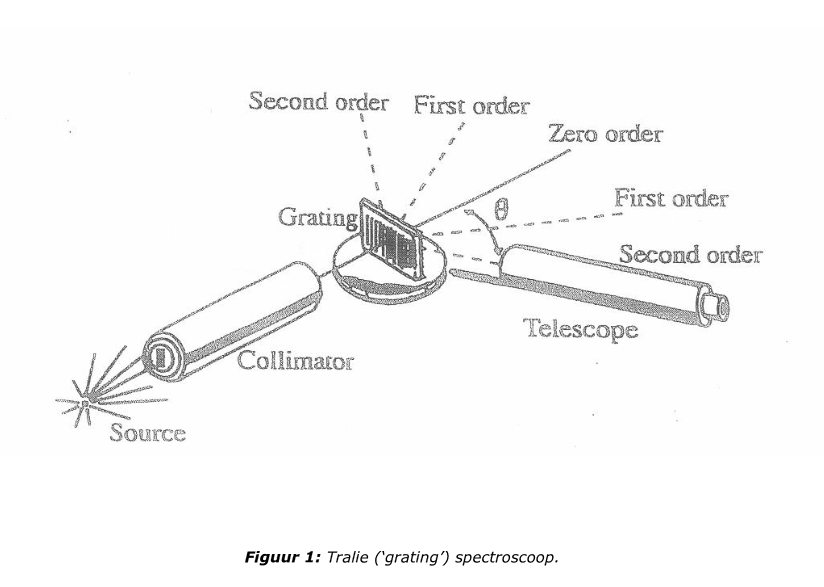
\includegraphics[width=1\linewidth]{afbeelding.png}
    \label{fig:enter-label}
\end{figure}